% Book general formatting, may need to adjust for printing
\documentclass[a5paper,twoside,openany]{book}
\usepackage[body={12cm,18cm}]{geometry}
\usepackage[a5,center,off]{crop}
\pagestyle{plain} % Remove chapter reminders on headers (book style)
% End book formatting

\usepackage{titlesec}
\usepackage{bbding}
\usepackage{amssymb,graphicx}
\usepackage{enumitem}
\usepackage{caption}
\usepackage{wrapfig}
\usepackage{lipsum}
\usepackage{kantlipsum}

\usepackage{hyperref}	% Makes table of contents clickable on the pdf, really unnecesary
\hypersetup{ 			% Makes table of contents clickable on the pdf
    colorlinks,
    allcolors=black,
}

\graphicspath{ {./images/} } % Set the path for the images


% NORMALIZE: Custom command to get "out of" a bullet list, to add normal paragraphs
\newcommand\vcent[1]{\vcenter{\hbox{#1}}}
\newenvironment{normalize}{\leftskip-\leftmargin}{\par}
\newcommand\loudspeaker[1][3]{\ensuremath{\vcent{\rule{.6ex}{.6ex}}\kern-.5ex%
  \vcent{\scalebox{.6}[1]{\rotatebox[origin=center]{90}{$\blacktriangle$}}}%
  \ifnum#1>0\relax\kern.1ex\vcent{\scalebox{.3}{)}}\ifnum#1>1\relax\kern-.15ex%
  \vcent{\scalebox{.4}{)}}\ifnum#1>2\relax\kern-.23ex\vcent{\scalebox{.5}{)}}%
  \fi\fi\fi}%
}
% END NORMALIZE

\begin{document}


\setlength\parindent{0pt} % Remove the space after paragraph titles, excessive by default

\titleformat{\chapter}[block] % Remove the "CHAPTER" descriptor, add number to title
  {\normalfont\huge\bfseries\centering} % Format for chapter title: huge font, bold
  {\thechapter} % Include the chapter number (e.g., "1")
  {1em} % Spacing between the chapter number and the title
  {} % Text before the chapter title (e.g., "Chapter 1 Title")

% Reducing title and section spacing  
\titlespacing*{\chapter} {0pt}{0ex}{0ex}

% Customizing the Table of Contents title
\renewcommand{\contentsname}{\small Sumario}
\renewcommand{\chaptername}{\small Capítulo}

% Title Page (optional, change later and put a real title page, with pictures and raccoons)
\title{%
	Guía para aprender a reparar tus propios aparatos electrodomésticos y electrónicos\\
	\small (¡incluso si nunca has cogido un destornillador!)
	}

\author{%
	David M. \\
	\small Asociación \\ 
	"l'Ateliéphémère"  \\\\
	Traducción: RestartersVLC \\
	}

\maketitle

\tableofcontents
\newpage
 

% Example content
\chapter{Introducción}
\section{Presentación de L'ateliéphémère}

L'ateliéphémère es una asociación que ofrece talleres (así como cursos de formación sobre temas específicos) para ayudarte a aprender a reparar tus propios
equipos eléctricos y electrónicos, electrodomésticos, etc.\\

\textbf{\underline{¿Cómo funciona?}}

Alguien trae su electrodoméstico averiado, explica el problema y juntos intentamos repararlo.

Pero como siempre aprendemos mejor haciéndolo nosotros mismos, es la persona que ha traído
la persona que ha traído el aparato utilizará las herramientas disponibles in situ.
herramientas.

El objetivo de estos talleres es demostrarnos a nosotros mismos que somos capaces de
reparar muchas cosas uno mismo con muy pocos conocimientos y
conocimientos técnicos.

Todo el mundo es capaz de cambiar un fusible o poner un poco de aceite
¡en el lugar correcto!

Mis años de estudiante de electrónica no me enseñaron gran cosa que fuera útil para reparar un electrodoméstico, aparte de aprender a soldar y el vocabulario para investigar más fácilmente
después.

Esta guía te ayudará a sentirte más tranquilo cuando te enfrentes a un aparato que diagnosticar.
diagnosticar un aparato, sin tener que dedicar años de minucioso estudio
años de estudio o leer tediosamente libros de texto teóricos llenos de complicadas
¡complicadas fórmulas que no le ayudarán a arreglar su batidora!
Por supuesto, hay mucha información que no está ahí, pero hay enlaces a ella.
pero hay enlaces a una serie de foros al final de esta guía para ayudarte a
para ayudarte a encontrar más información.

Y si vives en la región Rhône-Alpes, estos talleres tienen lugar actualmente en
en Saint-Étienne, Grenoble y Lyon (y ocasionalmente más lejos), en centros sociales
en centros sociales, talleres comunitarios de ciclismo, bares comunitarios, etc.
La antigüedad de estos talleres nos permite llegar a personas que están
acostumbradas a los lugares donde se celebran los talleres y que, por tanto, se sienten cómodas
se sienten cómodos acudiendo sin demasiada aprensión.
No creo que baste con decir que un lugar está "abierto a todos".
para que vengan personas alejadas de ciertas redes (asociaciones, activistas, etc.).
¡que vengan!

\section{¿Por qué la realización de esta guía?}
En primer lugar, porque, que yo sepa, no existe ningún folleto o libro destinado a explicar de la forma más sencilla posible lo que hay que hacer.
explicar de la forma más sencilla posible lo que hay que saber para empezar a
a reparar la mayoría de los aparatos que nos rodean.

Existen libros sobre el tema, que pueden ayudar con las reparaciones, pero son demasiado técnicos  y, por tanto, de difícil acceso si no se tiene un mínimo de conocimientos en la materia.
El objetivo de esta guía es, por tanto, explicar los fundamentos esenciales de la electricidad
y, a continuación, los conocimientos y consejos que le permitirán iniciarse en la
reparación de un electrodoméstico.\\

He intentado mantener la sencillez y no explicar demasiadas cosas complejas que
que no te servirían de nada a la hora de reparar un electrodoméstico. Me he inspirado en casos
encontrados en mis talleres que reflejan las averías más comunes.
He enmarcado pasajes que he escrito a título informativo pero que no son
esenciales, por ejemplo las fórmulas, que rara vez se utilizan para Ce
diagnosticar una avería.
Por tanto, estos pasajes están ahí para los más curiosos.

Si no lees esta guía desde el principio, puede que no entiendas de qué estoy hablando.
entender de qué estoy hablando.
Como mínimo tendrás que leer el capítulo 2 sobre los fundamentos de la electricidad para poder
entender cómo probar cada uno de los componentes.\\

Esta guía no requiere ningún conocimiento ni habilidad. Está dirigida a cualquier persona que
personas que prefieren tomarse el tiempo de desmontar un aparato y ver
lo que ocurre en su interior, en lugar de tirarlo y comprar uno nuevo
y contribuir así al enorme despilfarro que se está produciendo.

\section{Sobre las consecuencias de la electrónica}

Para fabricar un chip de 2 gramos se necesitan 1,6 kg de energía fósil, es decir
600 veces su peso. Los ordenadores y todos los productos electrónicos y eléctricos
Los productos eléctricos plantean graves problemas al final de su vida útil.
Según Serge Latouche, en su libro "Bon pour la casse", actualmente
150 millones de ordenadores son transportados cada año a vertederos ilegales en el
vertederos ilegales del Tercer Mundo (500 barcos al mes salen hacia Nigeria y
Ghana).
En los documentales de Cosima Dannoritzer "Prêt à jeter" y "La tragedia", nos enteramos de que el 75\% de esta basura electrónica no se recicla.
La mayor parte es quemada por niños en enormes vertederos al aire libre para recuperar los
recuperar metales raros.

\textit{"Se calcula que, en el mundo desarrollado, alrededor del 75\% de estos residuos desaparece de los circuitos oficiales de reprocesamiento. Gran parte se exporta ilegalmente, a vertederos clandestinos en África".
}\\
(http://greenfocusmag.com/ verite-e-waste-monde-afrique)

Por su composición, la electrónica es en cualquier caso muy complicada de reciclar.

Además de estos residuos, el \textbf{80\% de la electrónica mundial} se fabrica
en las fábricas de Foxconn en Shenzhen (subcontratistas de Apple, Acer, Blackberry
Dell, Google, Motorola, Toshiba, Asus....).

Esta "ciudad factoría" emplea a 1,4 millones de personas que trabajan 12 horas al día
día, 6 días a la semana por unos 150 euros.
En el primer semestre de 2010, se produjeron 14 suicidios en esta
fábrica. La principal respuesta a estos suicidios fue la instalación de redes "a prueba de suicidas" bajo el tejado de la planta.

(Leer en "La machine est ton seigneur et ton maître", publicado por Agone)

\section{Las 5 principales barreras para la reparación}
\begin{enumerate}
\item Falta de confianza en la propia capacidad de reparación.
Desde una edad temprana, las pantallas y los teclados están sustituyendo a las herramientas manuales.
\item El deseo de la industria de que los aparatos sean difíciles de
difíciles de desmontar: diseño "futurista", tornillos especiales o ausencia total de tornillos (moldeado, pegado, etc.).
\item La documentación técnica y los diagramas necesarios para comprender cómo funciona el
funcionamiento del equipo no se encuentran en ninguna parte.
\item Las piezas de repuesto ya no se fabrican o se fabrican a precios desalentadores.
precios desalentadores.
\item La publicidad que intenta convencernos de que necesitamos el nuevo modelo "más eficiente", "menos contaminante" (desperdiciar menos para contaminar menos...).
El resultado es lo que se conoce como "obsolescencia simbólica".
En 2002, más de 130 millones de teléfonos móviles en funcionamiento
se desecharon en Estados Unidos (Serge Latouche, "Bon pour la
Casse")
\end{enumerate}

\section{¿Y esto, se repara?}
En teoría, todo se puede reparar, pero en la práctica, sólo el 50\% de los aparatos (de todo tipo) salen de mis talleres en buen estado.
Principalmente por las barreras 2, 3 y 4 mencionadas anteriormente.
Además, con la llegada de los aparatos portátiles/desechables (teléfonos, tabletas, etc.)
que son cada vez más difíciles de reparar sin herramientas específicas, evolucionan demasiado rápido
para que la reparación sea una opción real.

\section{Pequeños consejos antes de comprar un aparato}
\begin{itemize}
\item ¿Realmente lo necesitas?
\item ¿Puedes pedirlo prestado ocasionalmente a amigos y familiares
o a través de redes de autoayuda: SEL, Accorderie, etc.
\item Compra de segunda mano: comprar una máquina de coser o una batidora de los
una máquina de coser o una batidora de los años 70 y 80 será, por lo general, mucho más robusta que los equipos actuales. También es más fácil de reparar porque suele ser diseño sencillo y sin artilugios electrónicos...
\item El hecho de que estos electrodomésticos hayan funcionado durante varias décadas demuestra su calidad.
\item Por desgracia, el precio de un aparato no siempre refleja su calidad.
calidad, pero lo más barato no suele sorprender por su larga
vida. Algunas marcas siguen siendo populares hoy en día. 
Pide información a tus conocidos expertos en la materia.
en este campo o en internet (aunque algunas marcas se hagan pasar por
algunas marcas se hacen pasar por consumidores en foros...).
\item Evita los equipos multifunción, los equipos compactos de alta fidelidad, las impresoras-escáner, etc. Suelen ser más complejos de desmontar y reparar. Y además, en caso de avería irreparable, se verá obligado a sustituir toda una parte de la que aún funciona.
¿Es realmente prioritario ahorrar espacio?
\item Evita los electrodomésticos con artilugios prácticos: son prácticos, pero se estropean más a menudo. La electrónica, a menudo inútil, ha colonizado en detrimento de la sencillez y la robustez.
Tomemos el ejemplo de un coche. ¿Adivina qué partes se averían más a menudo?

$\Rightarrow$ \textbf{Elevalunas eléctricos, apertura centralizada, sensores electrónicos, sensores de todo tipo...}

\item Evita también los dispositivos portátiles y miniaturizados.
¿Realmente necesita un ordenador portátil cuando durará mucho menos que un ordenador de sobremesa fijo que puedes puedes comprar por casi nada y cuyas piezas son fáciles de sustituir?
También será posible hacerlo más potente a menor coste.

\item También debe desconfiar del diseño y los electrodomésticos con
formas futuristas. Asegúrese de comprobar la presencia de tornillos "clásicos" para los que posee la herramienta. 

\item La mayoría de las tabletas y los teléfonos inteligentes, son dispositivos "desechables", muy frágiles y difíciles de reparar por uno mismo Además, la obsolescencia simbólica incita a sustituirlos por modelos más "eficientes". Vivimos muy bien sin estos aparatos "hiperconectados" que nos desconectan de la realidad.

\item Por último, evite comprar impresoras de inyección de tinta con escáner incorporado. Se trata de aparatos desechables, los cartuchos cuestan el precio de la impresora en venta, suelen imprimir mal y consumen mucha energía. Además consumen mucha tinta para limpiar regularmente los cabezales de impresión. Como prueba de su mala calidad, consigo cartuchos nuevos prácticamente en cada taller...

Es más, algunos modelos recientes de modelos de impresora-escáner: no podrás no podrás escanear ¡si la impresora se queda sin tinta! Decántate por las impresoras láser, más caras de comprar pero más económicas después. Esta tecnología es fiable y existen modelos B\&N de segunda mano a partir de 10 euros en Internet.

\begin{figure}[h]
    \centering
    \begin{minipage}[b]{0.4\textwidth}
        \centering
        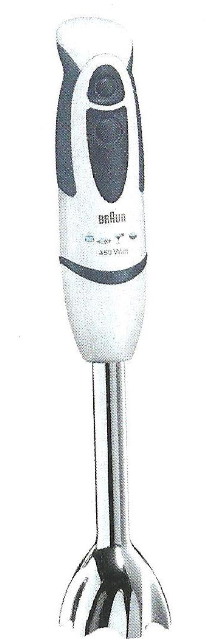
\includegraphics[width=0.3\textwidth]{braum-mixer} 
        \caption*{Ganador del concurso de batidoras indesmontables... Braum y Kenwood!}
    \end{minipage}
    \hfill
    \begin{minipage}[b]{0.4\textwidth}
        \centering
        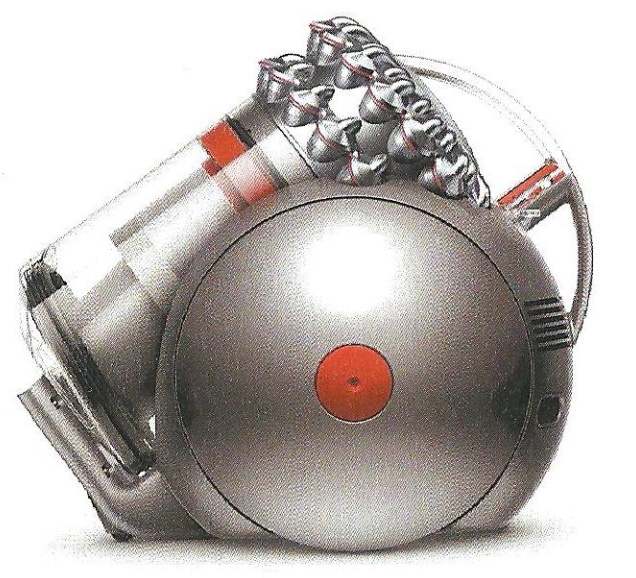
\includegraphics[width=\textwidth]{Dyson} 
        \caption*{¿Es para aspirar polvo intergaláctico?}
    \end{minipage}
\end{figure}



\end{itemize}


\chapter{Las bases de la electricidad}
\section{¿Qué es la electricidad?}
Con un poco de teoría, voy a explicar algunos conceptos básicos
para que entiendas lo que es la electricidad.
Así podrás medir y probar muchos de los componentes de tus
en tus electrodomésticos.

\begin{figure}[h]
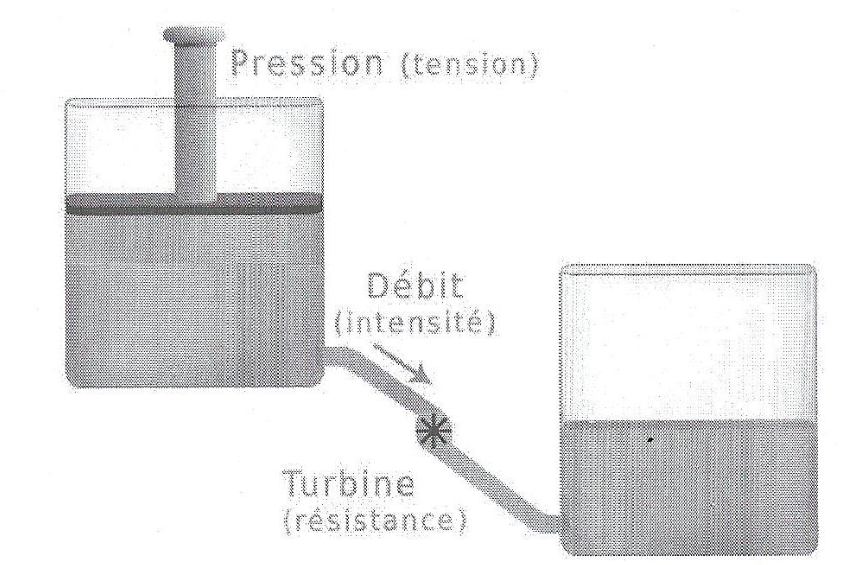
\includegraphics[width=0.8\textwidth]{analogia-agua-elec} 
\caption*{Analogía entre la electricidad y el agua}
\end{figure}

\begin{itemize}
\item \textbf{La tensión (U)} se expresa en voltios (V). Puede ser \textbf{Contínua}, como en una batería, salida del cargador, etc.) o \textbf{Alterna} (señales de la red eléctrica
señales electrónicas, etc.). Es una diferencia de potencial eléctrico entre dos
dos puntos. Siempre medimos una tensión entre dos puntos. Veremos más tarde cómo hacerlo. La tensión de una batería puede ser de 1.5V, 3V, 9V, la tensión de red ronda actualmente los 230V.

\item \textbf{La intensidad (I)} (o "corriente") se expresa en amperios (A).
Flujo de electrones a través de un hilo conductor con una determinada impresión.
A diferencia de la tensión, para que exista una corriente debe consumirse energía.
debe consumirse energía. ë
No hay corriente medible en una pila que no está conectada a nada.
- En este caso, decimos que no tiene "carga" (lo que no significa que no esté cargada en el sentido de que no esté conectada a nada).
 que no esté cargada en el sentido de una pila descargada, significa que
que no está suministrando energía).

\item \textbf{La resistencia (R)} se expresa en ohmios $\Omega$. Es muy baja
(a menudo se considera nula) para los metales y muy alta para el aire
el aire, el plástico o la madera seca, por ejemplo.
Por tanto, un cable eléctrico tendrá una resistencia muy cercana a 0$\Omega$ y el aire tendrá
una resistencia considerada infinita.
Algunos componentes electrónicos o elementos eléctricos también se denominan "resistencias"
o elementos eléctricos (por ejemplo, la resistencia de un horno eléctrico
horno o tostadora).
También existen resistencias "variables", ya sea por acción mecánica o por un cambio de temperatura.
o por un cambio de temperatura, por ejemplo.

\end{itemize}

\noindent\fbox{%
    \parbox{\textwidth}{%
La relación entre estos tres valores es $U(V) = R(\Omega) \times I(A)$, lo que implica que para una tensión fija, si disminuye la resistencia, la intensidad aumenta, y vice versa. Esto se comprende bien gracias al esquema de analogía entre el agua y la electricidad!
    }%
}\\

Para medir estos tres valores eléctricos, necesitamos una herramienta especial llamada "multímetro". (véase el capítulo 2.4).

\begin{figure}[h]
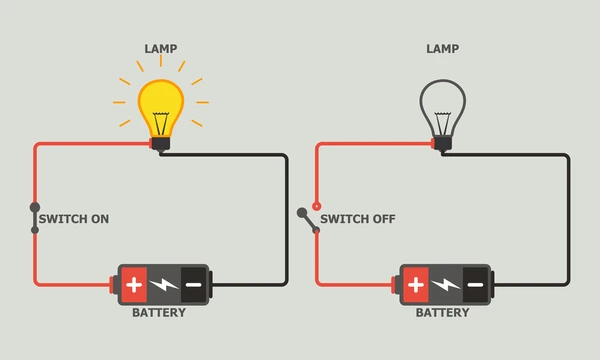
\includegraphics[width=0.7\textwidth]{circuito-abierto-cerrado} 
\centering
\caption*{Circuito abierto o cerrado (cambiar por otra figura)}
\end{figure}

\begin{enumerate}
\item Interruptor cerrado: la tensión "U" es igual a la tensión del generador, y ésta se extiende hasta los contactos de la lámpara (la tension en los extemos de un cable o de un interruptor cerrado siempre es de 0V). La corriente (I) existe y proporciona corriente a la lámpara para encenderse.
\item Interruptor abierto: la tensión "U" es igual a la tensión del generador, La tensión en los contactos de la lámpara es de 0V, no circula corriente
\end{enumerate}
La analogía con el agua no funciona aquí: un circuito cerrado significa que la electricidad puede circular.
posible circulación de electricidad, mientras que un grifo cerrado significa que no hay
circulación de agua...

\section{Los dispositivos de seguridad eléctrica}

\begin{large}
\textbf{a) Hilos y colores}\\
\end{large}
En primer lugar, para orientarse más fácilmente, hay que saber a qué corresponden los
corresponden en electricidad,
Pero como estos colores no siempre se respetan, veremos más adelante cómo estar seguros.
\begin{enumerate}
\item Para una tensión contínua:
\begin{itemize}
\item El hilo negro será el \textbf{-} (O a menudo el conector exterior en cables blindados)
\item El hilo rojo será el \textbf{+} (O a menudo el hilo conductor interior en cables blindados)
\end{itemize}


\begin{normalize}
Un cable "blindado" es un cable que está envuelto en un blindaje metálico conectado a la masa del aparato, para evitar interferencias electromagnéticas.
\end{normalize}

\item En lo que incumbe a instalaciones eléctricas: no se deje engañar por la posición del neutro y lugar del neutro y la fase en una toma eléctrica, esta norma no siempre se
esta norma no siempre se respeta, ya que si invierte el neutro y la fase, también
también funcionará.

\begin{figure}[h]
    \centering
    \begin{minipage}[b]{0.45\textwidth}
        \centering
        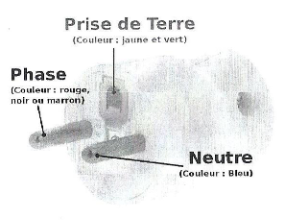
\includegraphics[width=\textwidth]{enchufe-macho} 
    \end{minipage}
    \hfill
    \begin{minipage}[b]{0.45\textwidth}
        \centering
        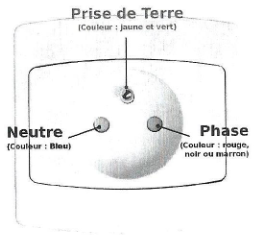
\includegraphics[width=\textwidth]{enchufe-hembra} 
    \end{minipage}
\end{figure}

\begin{itemize}
\item La fase (llegada de la corriente): todos los colores excepto azul y verde/amarillo. Puede estar directamente conectada al tablero de fusibles, o conecetada a un interruptor, por ejemplo
\item El neutro (escape de la corriente): azul
\item La tierra: verde y amarillo
\end{itemize}

\end{enumerate}

\newpage
\textbf{b) ¿De qué sirve la tierra y el disyunctor diferencial?}\\
Es importante comprender la finalidad de estos dos elementos, que han sido
creados para reducir el riesgo de electrocución de las personas en caso de avería de un aparato, como una fuga de agua en una lavadora, por ejemplo (el agua es un buen conductor de la electricidad)

\begin{figure}[h]
\includegraphics[width=0.7\textwidth]{diferencial-protección-tierra} 
\centering
\caption*{\textit{Los diferentes grados de protección de una instalación eléctrica}}
\end{figure}

Imagine un contacto eléctrico entre un cable conectado a un potencial eléctrico peligroso
(como la red de 230 V) y la carcasa metálica de su frigorífico.
de su frigorífico.

\begin{itemize}
\item Caso de la primera imagen: sin tierra ni disyunctor diferencial.
Si un apersona toca el frigorífico, la corriente pasará por el cuerpo de ésta para retornar a la tierra (ya que la corriente de la red está referenciada a tierra y siempre busca volver a ella, un poco como si se sintiese atraída por ella).

\textbf{$\Rightarrow$ La persona se electrocuta}

\item Caso de la segunda imagen: el cable de tierra está presente, es decir
todas las partes metálicas de los aparatos eléctricos están conectadas eléctricamente a tierra, pero sigue sin haber interruptor diferencial.
Esta vez, si alguien toca el frigorífico, la corriente fluirá a través del cable de tierra Y a través del cuerpo de la persona.

\textbf{$\Rightarrow$ La persona se da un calambre}
\newpage

\begin{normalize}
La corriente será mucho menor en el cuerpo de la persona que en el cable de tierra, porque la resistencia eléctrica entre la mano y los pies de una persona es mucho mayor que la de un cable de cobre. Cuanto menor sea esta resistencia (dedos y pies mojados, sobre un suelo húmedo, etc.), mayor será la fuga a tierra. Más fuerte y, por tanto, más peligrosa será la corriente.
\end{normalize}

\item Último caso: incluso antes de que alguien toque el aparato averiado, el disyuntor diferencial detectará la fuga de corriente y cortará la corriente a toda la instalación eléctrica. Se trata de la famosa palanca o botón grande que suele colocarse junto al contador de la luz.

\end{itemize}

\begin{figure}[h]
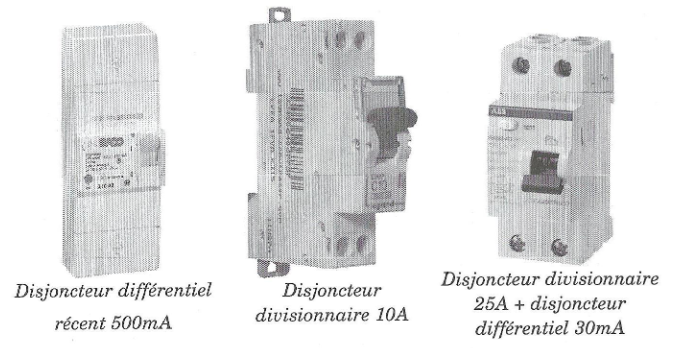
\includegraphics[width=0.9\textwidth]{disyunctores} 
\centering
\end{figure}

El interruptor diferencial mide la corriente que entra en la vivienda a través de la fase y la corriente que sale de la vivienda a través del conductor neutro.
Si la diferencia supera los 500 mA (650 mA en los modelos más antiguos), se dispara.
En ese caso, suele significar que un aparato conectado (no necesariamente en funcionamiento) está averiado.
Los interruptores diferenciales no deben confundirse con los interruptores divisionales.
disyuntores, que ahora sustituyen a los antiguos fusibles.\\

La función de un disyuntor divisor es cortar la electricidad a una parte de la instalación cuando se produce una sobreintensidad en dicha parte, es decir, cuando se produce un sobreconsumo anormal de corriente.
Generalmente, se disparan a los 16A para los enchufes convencionales, a los 10A
para el alumbrado (también los hay de 20A o 32A para alimentar determinados aparatos de alto consumo: cocina eléctrica, termo...).

La causa de esta sobreintensidad puede ser un aparato defectuoso, pero también puede ser el consumo normal de varios aparatos conectados al mismo circuito.
ser el consumo normal de varios aparatos conectados al mismo circuito de
circuito (no necesariamente el mismo enchufe).

\noindent\fbox{%
    \parbox{\textwidth}{%
Ejemplo: un termo eléctrico con una potencia P de 2300W, consumirá una corriente de 10A ($P = U \times I \rightarrow I = P/U = 2300W / 230V = 10A$)
Si enchufais uno o más aparatos sobre el mismo circuito, cuyo consumo sobrepase 6A, el disyunctor divisionario o el fusible de 16A cortará el circuito: $10+6=16A$
    }%
}\\

En las instalaciones recientes, se montan en el mismo módulo un disyuntor y un interruptor diferencial para cada parte de la instalación. Estos disyuntores diferenciales suelen dispararse a 30mA y por una buena razón:

\begin{figure}[h]
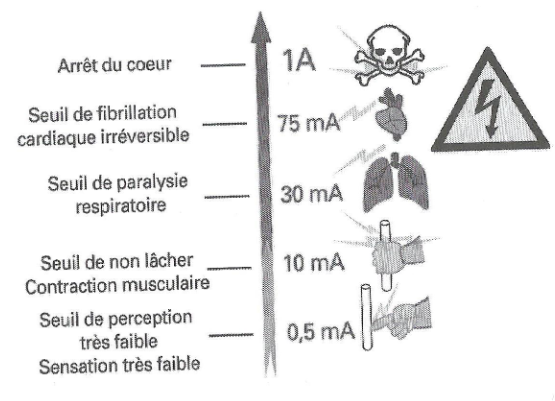
\includegraphics[width=0.9\textwidth]{corriente-efectos} 
\centering
\end{figure}

\textbf{b) ¿Cómo verificar una buena conexión a tierra?}\\
El disyunctor diferencial, está presente hoy en día en la mayor parte de instalaciones eléctricas de España, mientras que la toma de tierra está desgraciadamente ausente en muchas (la presencia de contactos de tierra en el enchufe no implica que esté conectada) Hay que coger el hábito de verificar si la tierra está bien conectada a los enchufes que vamos a usar para nuestros aparatos (sobre todo si hay facilidad de contacto con partes metálicas) Para ello, utilizaremos el multímetro (ver capítulo 2.4) en modo voltímetro en un rango de alterna superior a 240V.
\begin{itemize}
\item Entre el neutro y la fase deberíamos obtener 230V
\item Entre la fase y la tierra igualmente 230V (si no: tierra mal conectada)
\item Entre el neutro y la tierra, no más de 5V (si no: tierra mal conectada)
\end{itemize}
\newpage

Estas mediciones también permiten determinar la ubicación de la fase y el neutro, que no siempre están colocados como se muestra en el diagrama siguiente:

\begin{figure}[h]
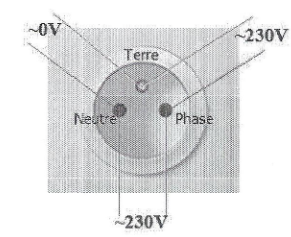
\includegraphics[width=0.4\textwidth]{diagrama-enchufe} 
\centering
\end{figure}

\section{Los peligros eléctricos que podeis encontrar durante las reparaciones}
Si no sabes lo que haces, la electricidad puede ser peligrosa e incluso mortal.
Al solucionar problemas, intentamos evitar trabajar bajo tensión en la medida de lo posible, pero el peligro no siempre se elimina. Me refiero a la tensión de red, los 230V AC. Sin embargo, un dispositivo alimentado por una batería también puede ser peligroso.\\

\textbf{a) Aparato bajo tensión}\\

Como norma general, conecte un aparato a la red sólo para una prueba o medición rápida y desconéctelo inmediatamente después.

\begin{itemize}
\item En caso de medir con el aparato bajo tensión, hay que poner especial atención a no poner los dedos, o cualquier parte del cuerpo en contacto con el aparato, las manos deben de estar sobre las dos puntas del multímetro y lo más alejadas posible de la parte bajo tensión.
\item No se debe tener ningún recipiente con agua u otro líquido a proximidad del aparato y la mesa de trabajo debe estar despejada y limpia.
\item Intentad estar lo más aislado posible del suelo, con buenos zapatos de goma e idealmente una tabla de madera debajo.
\end{itemize}
\newpage

\textbf{b) Aparato sin tensión o alimentado por una pila/batería}\\
Aunque el aparato esté desenchufado, debe tener especial cuidado con
un componente electrónico fácilmente reconocible: el condensador.
\begin{figure}[h]
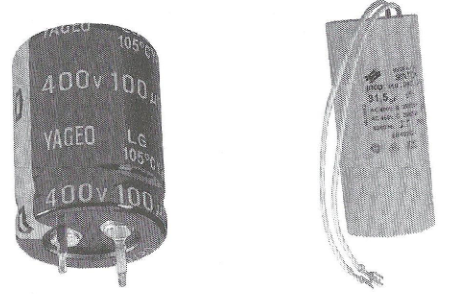
\includegraphics[width=0.7\textwidth]{condensadores} 
\centering
\end{figure}

Estos pequeños cilindros son capaces de almacenar alta tensión, lo que puede ser
peligroso.
Encontrará el modelo de la izquierda soldado a las tarjetas de alimentación de la mayoría de los aparatos más recientes conectados a la red que necesitan tensiones continuas. Pero también lo encontrarás en las cámaras digitales para dar al flash la potencia que necesita. El condensador de la derecha se encuentra en electrodomésticos como las lavadoras. También encontrará un condensador capaz de almacenar una tensión de unos 4000V en los hornos microondas: ¡una alta tensión muy peligrosa!
En ambos casos, la única forma de saber si debe desconfiar es
comprobar la tensión máxima admisible impresa en el componente.
Si supera los 50 V, deberá tomar las precauciones indicadas en el apartado
sección sobre condensadores (véase el capítulo 5.4.2).\\

En resumen, recuerde que los dispositivos potencialmente peligrosos, aunque estén apagados, son :
\begin{itemize}
\item Todos los aparatos alimentados por la red eléctrica equipados con una fuente de alimentación conmutada (véase el cap. 5.3.a)
\item Cámaras digitales
\item Hornos microondas
\item Tubos de rayos catódicos de pantallas y televisores antiguos
\end{itemize}
\newpage

\section{Utilización de un multímetro}
El multímetro es una herramienta electrónica esencial para medir
determinados valores eléctricos. La mayoría de los multímetros actúan como
voltímetro, amperímetro y óhmetro, es decir, miden tensiones
y resistencias, lo que suele bastar para la localización de averías.
resolución de problemas. La mayoría de las veces, lo único que necesitamos es medir tensiones y resistencias. Los multímetros se pueden adquirir por unos diez euros o más y son suficientes para la localización de averías.

\begin{figure}[h]
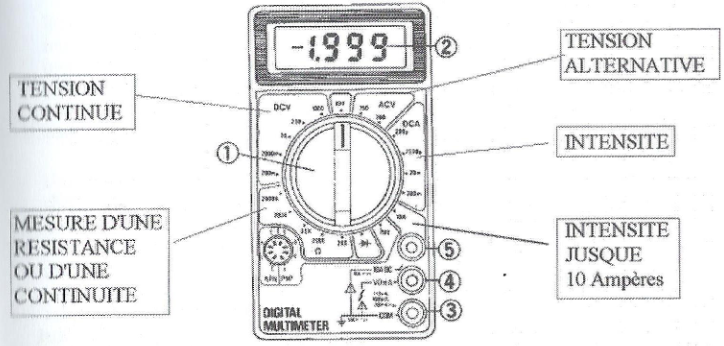
\includegraphics[width=\textwidth]{multimetro-digital} 
\centering
\caption*{\textit{Multímetro digital básico}}
\end{figure}
\textbf{a) ¿Cómo se utiliza?}\\

En primer lugar, con su multímetro, tendrá dos cables, uno rojo y uno negro. En un lado de estos cables, habrá una clavija "banana" que se conecta al multímetro, y en el otro lado, un "punto de contacto" para realizar las mediciones.
El negro se conecta siempre a la clavija "COM" (marcada con un 3 en la imagen) de su multímetro, el rojo puede enchufarse en diferentes puntos dependiendo de lo que quieras medir.
Ten en cuenta que por debajo de unos 50V (en un ambiente seco), no estás arriesgando mucho.
Puedes poner los dedos en los dos polos de una batería tanto como quieras. Sin embargo, ten mucho cuidado cuando estés midiendo tensiones más altas, como la de la red eléctrica, por ejemplo.

\newpage

\textbf{b) Medida de continuidad, de aislamiento y de resistencia}\\

Es muy importante saber medir la continuidad, de hecho es lo más importante
para encontrar la mayoría de los problemas en los equipos eléctricos.
equipos eléctricos.

Gracias a esta medida, podemos comprobar que la mayoría de los elementos eléctricos y ciertos componentes electrónicos.\\

Lo que llamamos "medir la continuidad" es comprobar que existe contacto eléctrico entre dos puntos.
La continuidad equivale a una resistencia prácticamente nula ($\approx$0$\Omega$).

En particular, se utiliza para comprobar que un cable no se ha cortado dentro de su aislamiento, lo que ocurre más a menudo de lo que se cree.
aislamiento, lo que ocurre más a menudo de lo que se piensa.

A la inversa, lo que llamamos "medir el aislamiento" es comprobar que
que no hay contacto entre dos puntos, es decir, que hay una resistencia "infinita".\\

\textbf{
Para medir la continuidad eléctrica o la resistencia, el aparato debe
estar siempre apagado}\\

El multímetro envía una corriente baja para realizar la medición.
Por lo tanto, esta medición es segura. Para comprobar la continuidad entre dos puntos, coloque el multímetro en el valor $\Omega$ más bajo o {\Large \loudspeaker}  si su multímetro dispone de la función "pitar para continuidad" (que le permite comprobar varias continuidades sin tener que mirar la pantalla cada vez).
Coloque sus dos puntas en los dos extremos a comprobar: si la continuidad es
Si la continuidad es buena, obtendrá un valor próximo a 00 y/o emitirá un pitido. Si no hay continuidad (resistencia demasiado alta), no cambiará nada en la pantalla. Mostrará OL (sobre límite) o "1" según el aparato.
Para comprobar la diferencia en pantalla entre continuidad y no continuidad, simplemente junte las dos puntas de su multímetro.Tenga en cuenta los diferentes prefijos: miliohm, ohm, Kohm, Mohm.\\

A veces será necesario comprobar una resistencia infinita.
(Por ejemplo, entre las clavijas que alimentan un elemento eléctrico y su carcasa metálica, debe haber una resistencia infinita).
Debe hacer lo mismo que para medir la continuidad, excepto que debe ajustar el multímetro al valor $\Omega$ más alto. No ajuste el multímetro a la función "continuidad" para esta medición.
El aislamiento se produce cuando no ocurre nada en la pantalla durante la medición.
\newpage

Para medir una resistencia eléctrica, sitúese sobre $\Omega$ y coloque las puntas en las extremidades de la resistencia, si obtiene una resistencia infinita, está cortada y necesita ser reemplazada.
Si obtiene 0 $\Omega$, puede estar en cortocircuito, así que desuelde/desenchufe la resistencia del resto del resto del aparato y mida de nuevo sus terminales para comprobar que está en cortocircuito. Si no es así, el problema está en otra parte del aparato: otra resistencia conectada en paralelo, por ejemplo.\\

\textbf{
c) Medida de la tensión}\\
Aparte de las señales electrónicas más complejas (cuadrada, triangular, modulada....), en las que no entraré en esta guía, hay dos formas de tensión que debes conocer: la tensión continua y la tensión alterna "sinusoidal" de la red eléctrica doméstica.

\begin{itemize}
\item \textbf{La tensión contínua}

\begin{normalize}
Una tensión continua es una tensión estable en el tiempo y que tiene una forma lineal
una pila de 9V (si no tenemos en cuenta que se descarga gradualmente) siempre entregará 9V. 
Para medir una tensión de este tipo, pon tu multímetro en tensión continua
(CC o V=). Si hay varios calibradores (algunos multímetros tienen calibración automática
calibración automática) y no sabe lo que va a obtener, elija el mayor; si obtiene algo como 0,001V, reduzca el calibre hasta que obtenga un valor bastante exacto.
A continuación, simplemente coloque cada una de las puntas de su multímetro sobre los dos contactos a medir, el + y el - de una pila, por ejemplo.
Si las patillas de su multímetro están invertidas, mostrará un "-" delante del
del valor.
\end{normalize}

\newpage


\item \textbf{La tensión alterna sinusoidal}
En contra a una tensión contínua, la tensión alterna tiene una evolución cíclica respecto al tiempo.

\begin{figure}[h]
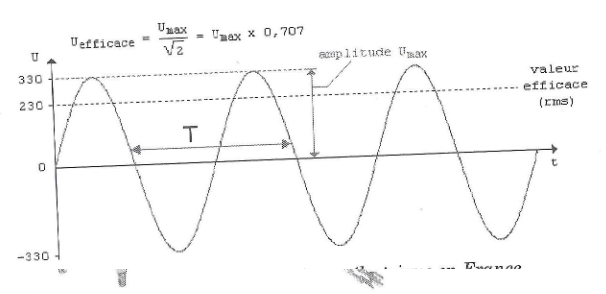
\includegraphics[width=\textwidth]{tension-alterna-sinusoidal} 
\centering
\caption*{\textit{Forma de la tensión de la red eléctrica europea}}
\end{figure}
Tomemos el ejemplo de nuestra red eléctrica, es una tensión sinusoidal de 230V, así que coloque su multímetro en "tensión alterna" (AC o V$\approx$), sobre el primer valor más alto que 230V
A continuación, basta con colocar cada una de las puntas del multímetro en uno de los dos contactos a medir, un enchufe por ejemplo. Si inviertes el + y el - en tu multímetro, no habrá ninguna diferencia. No hay "dirección" en una corriente alterna ya que cambia de dirección regularmente, lo que medimos es lo que llamamos su "valor eficaz".

\noindent\fbox{%
    \parbox{\textwidth}{%
Definición: El valor eficaz de la tensión (llamada "rms"), es el valor de una tensión contínua que tendría los mismos efectos sobre una resistencia eléctrica.
    }%
}\\


\noindent\fbox{%
    \parbox{\textwidth}{%
Esta señal se llama "alterna", porque cambia de signo/sentido, tiene un período (T) que determina la duración del patrón elemental que se reproduce al infinito. Este período (T) se mide en segundos, en la red eléctrica es de 0.02 segundos (s) o 20 milisegundos (ms).\\
Más a menudo hablamos de la frecuencia de una señal (Hercios), que está directamente ligado a el periodo, ya que equivale a su inversa: $ f = \frac{1}{T}, sea \frac{1}{0.02} = 50 Hz$ para nuestro ejemplo. La señal del tendido eléctrico Español es pues 50 Hz, es decir, se repite a una velocidad de 50 veces por segundo.
    }%
}\\
\end{itemize}
\newpage

\textbf{
d) Montaje en serie y en paralelo}\\

Ya sea en corriente continua o alterna, a veces oirás hablar de conexión en serie o en paralelo, son las distintas formas de conectar componentes eléctricos entre sí según sea necesario.
\begin{itemize}
\item En serie

\noindent\begin{minipage}[t]{0.5\textwidth}\vspace{0pt}
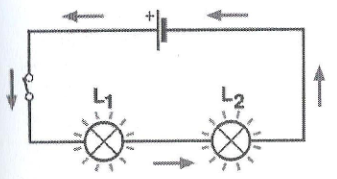
\includegraphics[width=\linewidth]{circuito-serie}
\end{minipage}% Don't leave empty lines and empty chars between minipages
\hfill%
\begin{minipage}[t]{0.45\textwidth}\vspace{0pt}
Montaje en serie significa que el
de tal manera que la misma corriente
la misma corriente pase a través de ellos
 uno tras otro.
La corriente es la misma en todo el
circuito, mientras que la tensión en
terminales de la batería es igual a la suma
de las tensiones en los bornes de cada
lámpara.
\end{minipage}

\item En paralelo (o en derivación)

\noindent\begin{minipage}[t]{0.5\textwidth}\vspace{0pt}
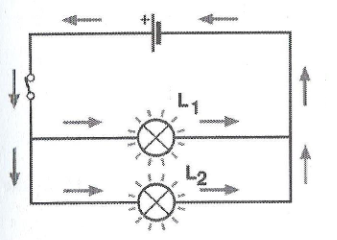
\includegraphics[width=\linewidth]{circuito-paralelo}
\end{minipage}% Don't leave empty lines and empty chars between minipages
\hfill%
\begin{minipage}[t]{0.45\textwidth}\vspace{0pt}
La conexión en paralelo significa que
los dos polos de cada elemento están conectados entre sí.
La corriente suministrada por la batería se
dividida en dos partes para cada una de las lámparas.
Sin embargo, la tensión en los bornes de cada lámpara es la misma que la de la batería.
\end{minipage}
\end{itemize}
Es importante entender la diferencia entre estas dos asociaciones de elementos (o componentes electrónicos) porque no se comprobarán estos elementos de la misma manera en ambos casos.
Por ejemplo, en conexión en paralelo, si mide un cortocircuito en los terminales de L1, quizás sea L2 y no L1 el que tenga la culpa. Deberá desconectar una de estas lámparas para comprobarlo.
\newpage

\chapter{Pasemos a la práctica}
En primer lugar, en lo que respecta a los equipos electrónicos, existe un documento técnico muy valioso para cada aparato: el manual de servicio.
Si tiene la suerte de encontrarlo en Internet (a veces gratis), le dará mucha información que le ayudará a entender su máquina.
La mayoría de las veces, le proporcionará: el esquema electrónico, el despiece
para facilitar el desmontaje, el valor de los componentes y sus números de pieza
los ajustes, los "códigos de error" y la información para entrar en el modo de diagnóstico, etc.

\section{Herramientas}
Esta es la lista de herramientas que utilizo en mis talleres:

{\large \textbf{a) Indispensables:}}
\begin{itemize}[label=\CheckmarkBold]
\setlength\itemsep{0em} % Reduce Vspace to make the list fit in the page
\item Destornilladores de todas las formas y tamaños, incluidos destornilladores planos y Phillips, así como tornillos TORX, que suelen utilizarse en electrodomésticos. 
\item Alicates: multiusos, de punta larga, de corte, de nariz de bruselas, etc. 
\item Llaves: planas, de vaso, ajustables... 
\item Un cúter 
\item Un multímetro, lo más básico posible, suele ser suficiente.
\item Un soldador, si crees que vas a soldar con regularidad, puedes permitirte pagar el precio y comprar calidad. Elige una punta de aproximadamente 1 mm de diámetro. 
\item Una esponja o lana de acero para limpiar la punta del soldador.
\item Una bomba desoldadora para aspirar la soldadura.
\item Una lupa
\item Una pera de aire para quitar el polvo (no te salpiques con botes de aire seco).
\item Un cuchillo para ostras: la mejor herramienta que he encontrado para desmontar aparatos con carcasas de plástico enganchadas. Te ahorrará la molestia de destrozar muchos destornilladores planos.
\item Un cable con un enchufe macho en un extremo (con toma de tierra) conectado a 3 conectores hembra "SPADE" en el otro extremo.\\
\end{itemize}

Este cable te será muy útil para conectar directamente aparatos electrodomésticos, puedes modificar un enchufe de algún aparato y soldar los conectores tú mismo.

\begin{figure}[h]
    \centering
    \begin{minipage}[b]{0.45\textwidth}
        \centering
        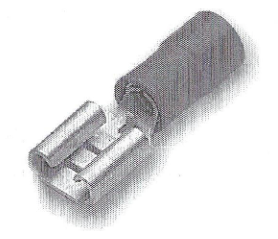
\includegraphics[width=\textwidth]{spade-female} 
        \caption*{Conector tipo "SPADE" hembra}
    \end{minipage}
    \hfill
    \begin{minipage}[b]{0.45\textwidth}
        \centering
        
\includegraphics[width=\textwidth]{torx-symbol} 
        \caption*{Tornillo Torx}
    \end{minipage}
\end{figure}

\vspace{1em}
{\large \textbf{b) Opcionales:}}
\begin{itemize}[label=\CheckmarkBold]
\setlength\itemsep{0em} % Reduce Vspace to make the list fit in the page
\item Una pistola de aire caliente, muy útil para reblandecer pegamentos, detectar fallos que se manifiestan cuando el aparato se sobre calienta, y para aplicar termoretráctil.
\item Una "tercera mano": brazos articulados con npinzas, y a veces una lupa, para soldar cómodamente.
\item Un tester de componentes electrónicos, se encuentran por 15€ en internet.
\item Un magnetizador/desmagnetizador de destornilladores, no son caros y permiten recuperar tornillos difícilmente accesibles...
\item Limas pequeñitas.
\item Pistola de cola caliente.
\item Pelacables.
\item Bomba de aire frío para detectar fallos que aparecen en función de la temperatura.
\item Una regleta con interruptor para apagar rápidamente aparatos "dudosos".
\end{itemize}
\newpage

{\large \textbf{c) Consumibles:}}
\begin{itemize}[label=\CheckmarkBold]
\setlength\itemsep{0em}
\item Varios tipos de pegamento (super glue, epoxy, etc.)
\item Trenza desoldadora.
\item Alambre de estaño de 0,5 y 1mm de diámetro.
\item Grasa.
\item Aceite de vaselina.
\item Alcohol de 90° o isopropílico (para la óptica).
\item Pegamento de "contacto" F2.
\item Lubricante anti-oxidante.
\item Tubo termorretráctil de varios diámetros.
\item Flux de soldadura.
\end{itemize}

\section{El desmontaje: el inicio de la lucha...}
En los electrodomésticos recientes, el desmontaje suele ser una etapa tan difícil como la propia reparación, a veces incluso más. Fabricantes, ingenieros y diseñadores innovan año tras año para asegurarse de que no podamos desmontar sus (¿nuestros?) aparatos.
Utilizar tornillos ocultos bajo las etiquetas, bajo las patas de goma o bajo las piezas de plástico clipadas a veces puede hacernos perder mucho tiempo. También encontrarás tornillos "de seguridad", comprar el destornillador para quitarlos puede valer una fortuna...
A veces, la ausencia de un tornillo significa que tendrás que buscar mucho tiempo para encontrar el lugar adecuado para abrir el aparato sin romperlo.
Y por último, los aparatos moldeados y pegados a veces obligan a utilizar un cúter a lo largo de una ranura para acceder al interior... (batidoras de inmersión Braun y Kenwood, cargadores Apple...) Sólo la perseverancia (y la ayuda de internet) harán que no te rindas antes de empezar...

Tómate tu tiempo para mirar las cosas, para intentar separar cada parte de las demás, para "sentir" cada parte. Intenta "sentir" qué se mueve y qué no se mueve en absoluto, para deducir si hay algún tornillo que no hayas encontrado.

\begin{figure}[h]
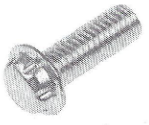
\includegraphics[width=0.2\textwidth]{tornillo-tostadora-phillips} 
\centering
\caption*{\textit{Tornillo extraño encontrado en tostadoras phillips}}
\end{figure}

Cuando se trata de destornilladores de diferentes formas y tamaños, puedes encontrar casi cualquier cosa en ifixit.com, pero una vez más, el precio de la herramienta comparado con el del aparato a reparar detendrá a mucha gente en su camino. Sólo la puesta en común de herramientas puede resolver este problema.\\

{\large \textbf{a) Cómo desatornillar:}}\\

La mayoría de la gente cree saber cómo desenroscar, sin embargo no es raro encontrar casos de gente que lo realizan de mala manera, lo que a veces es destructor para la cabeza del tornillo, y vuelve el desmontaje del aparato imposible sin un taladro de columna para hacer desaparecer la cabeza del tornillo con una broca, cosa que no todo el mundo tiene a su alcance...
Aquí hay un método para evitar esta situación:

\begin{itemize}
\item Elige la herramienta adecuada: fíjate bien en la forma del tornillo
coge un destornillador con la broca que te parezca más adecuada, colócalo en el tornillo y comprueba que no hay holgura entre la punta y el tornillo.
La punta debe acoplarse perfectamente al tornillo, casi no se debe ver holgura.
\item A continuación, aconsejo mantener un buen apoyo vertical sobre el tornillo y dar un pequeño golpe seco de rotación, en el sentido inverso de las agujas del reloj (excepto en casos raros: rotnillo sobre el eje de un motor, en algunas piezas de bici, máquinas de coser...)
De esta manera evitaremos al máximo que el destornillador "salte" sobre el tornillo y deteriore la cabeza, haciendo su extracción cada vez más difícil.
\end{itemize}
\begin{figure}[h]
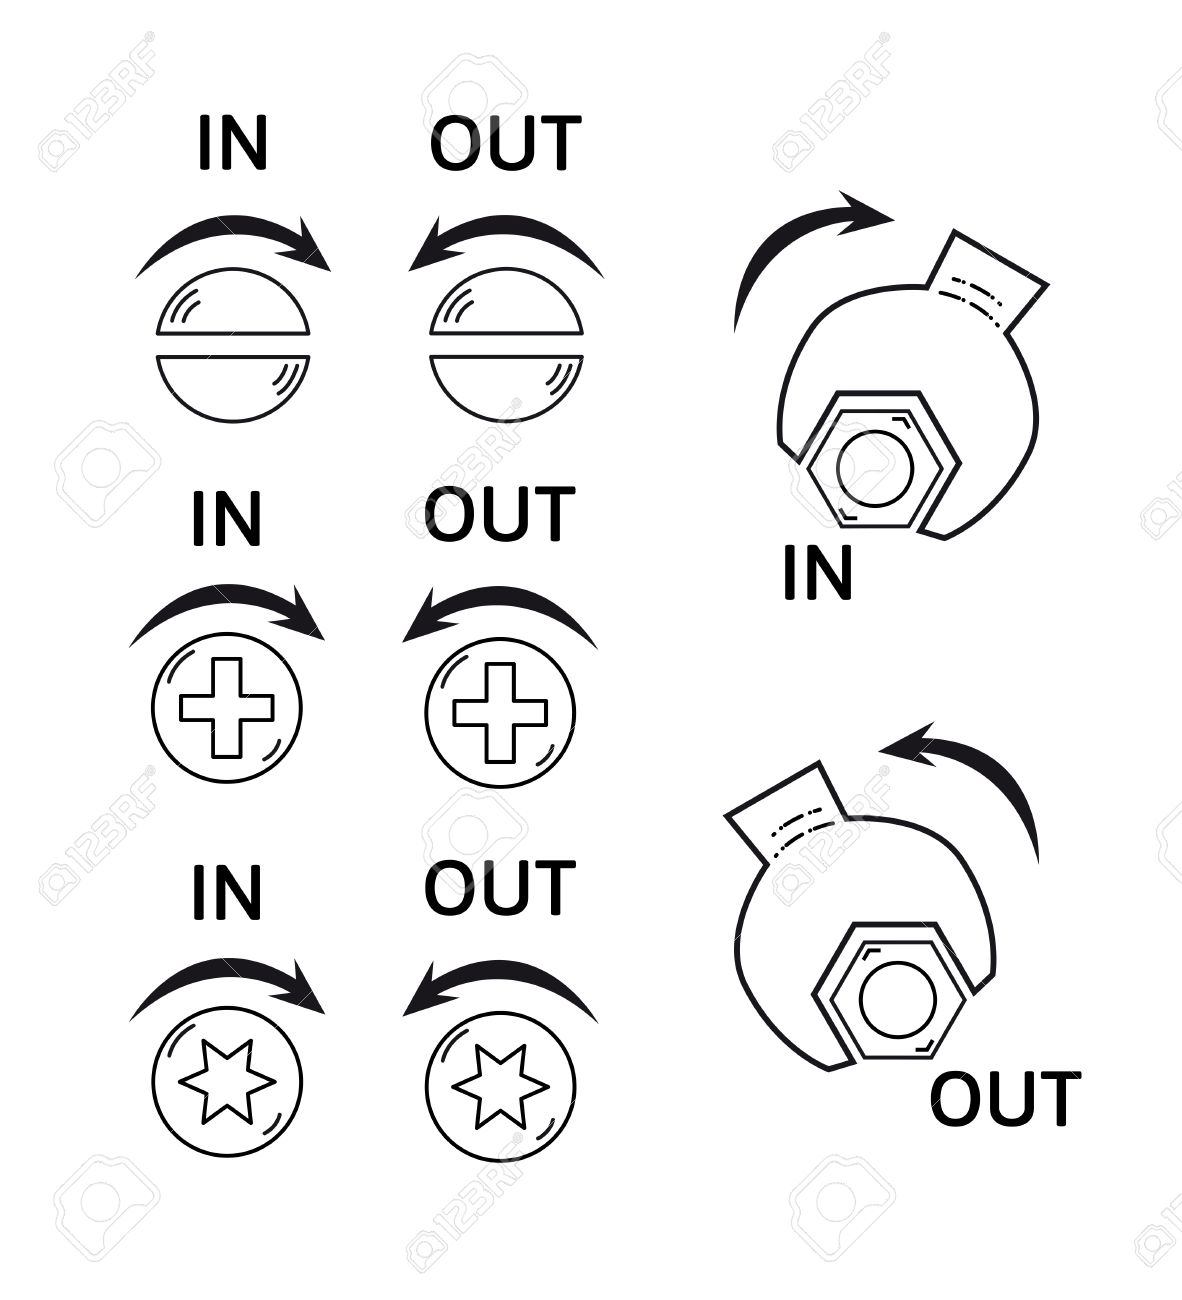
\includegraphics[width=0.4\textwidth]{diagrama-righty-tighty} 
\centering
\caption*{\textit{Righty tighty, lefty loosey ;)}}
\end{figure}

{\large \textbf{b) Los conectores:}}\\
Cuando desmontes u aparato, a menudo deberás desconectar placas electrónicas conectadas entre ellas, o conectadas por algún tipo de cable con conectores. A veces es suficiente estirar (a veces incluso con bastante fuerza), pero debes tener cuidado con ciertos conectores. Mira bien si no hay algún mecanismo de cerrojo como para los modelos encontrados abajo. A menudo, el clip de desconexión es de un color distinto al resto del conector.

\begin{itemize}


\begin{figure}[h]
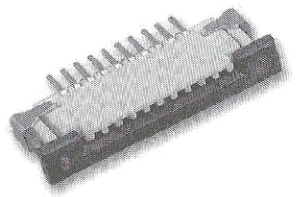
\includegraphics[width=0.4\textwidth]{conector-deslizante} 
\centering
\caption*{\textit{Modelo de conector deslizante}}
\end{figure}
\item Modelo deslizante: hay que tirar ligeramente hacia el exterior del mecanismo para desconectar el cable.
\begin{figure}[h]
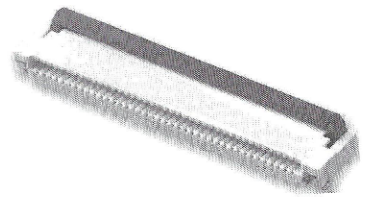
\includegraphics[width=0.4\textwidth]{conector-basculante} 
\centering
\caption*{\textit{Modelo de conector basculante}}
\end{figure}
\item Modelo basculante: hay que levantar delicadamente la parte superior del mecanismo, a veces del lado del cable, menos frecuentemente, como en la foto, del lado opuesto.
\end{itemize}

En ambos casos, usa las uñas o un destornillador plano muy fino y tira con cuidado, cuando se rompe un conector de este tipo suele ser bastante difícil de remplazar.
\newpage

\section{Historial y origen del problema}

Es muy importante enterarse del historial de un fallo para deducir de donde puede (o no) venir.\\

{\large \textbf{a) El aparato se ha caído o ha recibido un golpe}}\\

Si es así, es muy probable que algo se haya roto en el interior y esté causando una avería,
causando un mal funcionamiento: una placa de circuito rota o agrietada, un conector, un cable o una soldadura arrancados, un trozo de plástico roto...
El problema suele ser visible, sólo tienes que mirar con atención.
Con la práctica, serás capaz de ver enseguida qué falla.\\

{\large \textbf{b) El problema empeora cada día}}\\

Si la avería se ha producido gradualmente, hay que pensar en algo que evoluciona con el tiempo, acumulación de polvo, componentes al final de su vida útil, etc.
Según el tipo de electrodoméstico y avería, debe dar prioridad a la revisión de las partes que necesitan una limpieza regular:

\begin{itemize}

\item Los elementos ópticos: bloque lector de un CD/DVD
\item Los elementos y componentes que se calientan, y aquellos que los enfrían: disipadores y ventiladores de un ordenador portátil
\item Las partes mecánicas: barqueta de un lector CD/DVD, correas, engranajes...
\item Los contacos eléctricos: muelles de contacto de las pilas, interruptores, escobillas del motor...
\end{itemize}

{\large \textbf{c) El fallo aparece después de la puesta en marcha}}\\

En este caso, se trata probablemente de un elemento o componente electrónico cuyo estado cambia en función de su temperatura, por ejemplo
una unión soldada (porque el metal se dilata con la temperatura).

Puede tratarse de un componente mecánico cuya lubricación (demasiado antigua) mejora volviéndose más fina al aumentar la temperatura.

O al contrario, un componente eléctrico que funciona mal en cuanto sube la
temperatura.\\
\newpage
{\large \textbf{d) Problema intermitente}}\\

Si el problema aparece y desaparece sin ninguna razón en particular, o aparece cuando mueves el aparato, probablemente se trate de un mal contacto de una unión soldada o un conector.\\

{\large \textbf{e) El problema aparece en funciones específicas}}\\

Si el aparato se enciende, entiende comprender qué es lo que funciona y lo que no, ayudará mucho al diagnóstico que sigue.
Por ejemplo, prueba varios programas de la lavadora, si no deja elegir la función de centrifugado o vaciado de forma independiente a un programa, intenta ver si estas funciones pueden ser parte del problema (fallo de la bomba, fallo del elemento calentador ...)
A veces existen programas de diagnóstico, sobre todo en lavadoras y lavavajillas.
\newpage

\chapter{Electrodomésticos}
A continuación presentaré los principales componentes que se encuentran en los aparatos eléctricos y electrodomésticos.

\section{Los interruptores}
{\large \textbf{a) Interruptores, inversores y pulsadores}}\\

\noindent\begin{minipage}[t]{0.35\textwidth}\vspace{0pt}

El interruptor más básico es un sistema para cerrar y abrir un
circuito eléctrico, ya sea a tensión de red u otra señal eléctrica.
Su límite será la corriente que puede pasar a través de ellos sin
dañarlos.\\

\begin{flushleft}
Hay interruptores dobles que permiten abrir y cerrar dos circuitos
en paralelo y una variante conocida como conmutador que permite conectar un pin común a
cualquiera de sus otras dos patillas. Existen más complejos: triple,
cuádruple, etc. Pero el principio sigue siendo el mismo
\end{flushleft}
\end{minipage}% Don't leave empty lines and empty chars between minipages
\hfill%
\begin{minipage}[t]{0.6\textwidth}\vspace{0pt}
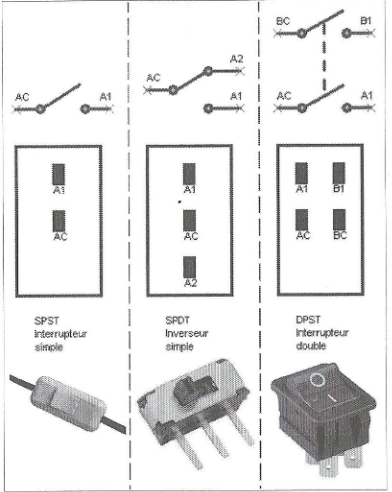
\includegraphics[width=\linewidth]{tipos-interruptores}
\end{minipage}
\vspace{1em}

Se comprueban simplemente con el multímetro en modo continuidad y aislamiento
(véase el capítulo 2.4.b).
\newpage

Otro tipo de interruptor que se encuentra generalmente soldado en placas electrónicas es el "botón pulsador", su particularidad es que sólo cierra el circuito mientras está pulsado, y lo abre al soltarse.
Existen de 2 y de 4 patillas, como en la foto, sin embargo las patillas están conectadas internamente 2 a 2 de cada lado y sólo es capaz de conmutar 1 circuito.

\begin{figure}[h]
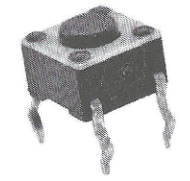
\includegraphics[width=0.25\linewidth]{boton-pulsador}
\centering
\end{figure}

Se encuentran encontrará detrás de cada botón de un equipo de alta fidelidad, reproductor de CD/DVD, ordenador portátil (aparte del teclado), pantalla, etc,
El popular modelo de arriba hace un pequeño "clic" al pulsarlo.\\

\textbf{Fallos comunes:}
\begin{itemize}
\item Mal contacto eléctrico interno, que provoca una alimentación intermitente o chispazos (en pulsadores no):
\\

$\blacktriangleright$ Si puedes desmontar la pieza (es el caso sobre todo de los interruptores como el anterior), intenta comprender qué partes que partes necesitan hacer contacto. En los interruptores que controlan la tensión de red, suele ocurrir que en el punto preciso
donde se hace el contacto, el metal está ennegrecido e impide un buen contacto eléctrico.
En este caso, a menudo basta con limpiar con una pequeña lima o papel de lija para restablecer un buen contacto eléctrico, seguido de una limpieza con alcohol de 90° o spray "limpia contacto".
\\

En el caso de los interruptores pequeños o pulsadores que no se pueden desmontar, echar limpiacontactos puede ser suficiente para darles una nueva vida. Si no, han de ser reemplazados, suelen ser muy baratos.

\item Ausencia de contacto
\\

$\blacktriangleright$ Si puede desmontarse, comprueba que no se ha movido ninguna pieza del interior.
A menudo habrá que sustituir toda la pieza.
\\
\end{itemize}
\newpage

\textbf{b) Un interruptor particular: el temporizador}

\noindent\begin{minipage}[t]{0.5\textwidth}\vspace{0pt}
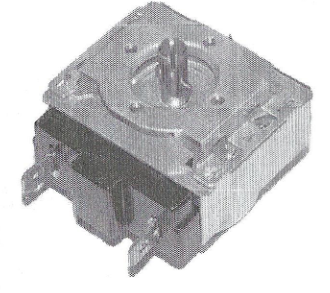
\includegraphics[width=\linewidth]{temporizador}
\end{minipage}
\hfill%
\begin{minipage}[t]{0.4\textwidth}\vspace{\fill}
\vspace{\fill} % Add this to push the text down
Es un interruptor, excepto que se utiliza para cerrar el circuito,
que se abrirá de nuevo cuando haya transcurrido el tiempo deseado.
Se prueba como un interruptor simple.
\vspace{\fill} % Add this to push the text down
\end{minipage}
\vspace{1em}

\section{Sensores}

Un sensor es un elemento que recibe y transmite una información: posición de un elemento (por diferentes métodos: mecánica, óptica, magnética...), movimiento, temperatura, presión...

Transmite esta información de forma eléctrica (interruptor abierto/cerrado, resistencia variable).

Algunos sirven directamente para cotar la alimentación eléctrica.
Otros, como el sensor de efecto hall, requieren otros componentes electrónicos para ser interpretados.\\

\begin{center}
\textbf{a) Sensores de posición mecánica}
\end{center}
\begin{minipage}[h]{\textwidth}\vspace{0pt}
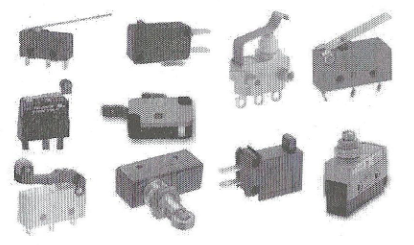
\includegraphics[width=0.6\linewidth]{sensores-posicion-mecanica}
\centering
\end{minipage}

Se encuentran en muchos aparatos, pueden servir para verificar si una puerta está bien cerrada (horno microondas) o la presencia de una tapa/recipiente (batidora, blender)
\newpage

A menudo están cableados en serie (véase cap. 2.4.4) con la alimentación del elemento potencialmente peligroso (motor que hace girar las cuchillas, etc.).
Es una fuente de averías muy frecuente. Suele tener 2 ó 3 clavijas:

\begin{itemize}
\item 2 patillas, es un interruptor clásico, verifica que esté en modo abierto (sin continuidad) en la posición "OFF" y en posición cerrada (con continuidad) en la posición "ON".
\item 3 patillas, es un conmutador. Tiene 3 patillas llamadas Reposo, Trabajo y Común.
\end{itemize}


\noindent\begin{minipage}[t]{0.35\textwidth}\vspace{0pt}
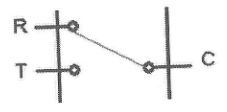
\includegraphics[width=\linewidth]{conmutador}
\end{minipage}
\hfill%
\begin{minipage}[t]{0.6\textwidth}\vspace{\fill}
\vspace{\fill} % Add this to push the text down
Cuando está en posición de reposo (obligado por un muelle, cuando no hay presión): Hay contacto entre la patilla C y R, y no hay contacto entre la T y las 2 otras.\\
\vspace{\fill} % Add this to push the text down
\end{minipage}
\vspace{1em}

Cuando está en posición de trabajo, C y T están en contacto y no hay contacto entre R y las otras 2.

A menudo hay que deducir a qué corresponde cada patilla, ya que no siempre están etiquetadas. Verifica bien que no haya ningún cortocircuito indeseado, ni ningún circuito abierto indeseado según la posición, y que los estados conmutan al accionar el conmutador.

\begin{center}
\textbf{b) Sensores de temperatura}
\end{center}

\begin{itemize}

\item El termostato mecánico regulable

\noindent\begin{minipage}[t]{0.45\textwidth}\vspace{0pt}
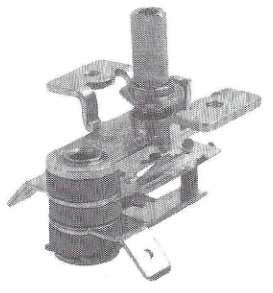
\includegraphics[width=\linewidth]{termostato}
\end{minipage}
\hfill%
\begin{minipage}[t]{0.5\textwidth}\vspace{\fill}
\vspace{\fill}
No es ni más ni menos que un interruptor
que se abre y se cierra en función de la
temperatura deseada.

Se trata de una función muy común en
electrodomésticos: hornos, planchas, calentadores eléctricos
plancha, calentador eléctrico, placa
hornillos, etc.

Se comprueba del mismo modo que un interruptor.
Oirá un pequeño "clic" cuando se enciende el termostato. Este chasquido suele significar que está funcionando correctamente.\\
\vspace{\fill}
\end{minipage}
\vspace{1em}
\\

\item El klixon

\begin{normalize}
\begin{minipage}[h]{\textwidth}\vspace{0pt}
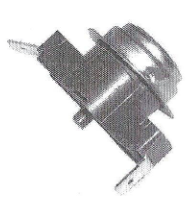
\includegraphics[width=0.3\linewidth]{klixon}
\centering
\end{minipage}

Se trata de un seguro térmico. 
Se encuentra por ejemplo en lavadoras, en el interior de la cuba.
Cuando la temperatura sobrepasa cierto límite, se abre y corta la corriente.
Cuando es rearmable, suele tener un botón que permite volver a conectarlo (hasta la próxima vez que se exceda la temperatura)

Cuando ocurre un sobrecalentamiento suele ser por un fallo del termostato, que no ha regulado bien la temperatura del aparato y ha provocado un sobrecalentamiento.
El klixon se testea con el modo continuidad.
\end{normalize}

\item La sonda térmica

\begin{normalize}
\begin{minipage}[h]{\textwidth}\vspace{0pt}
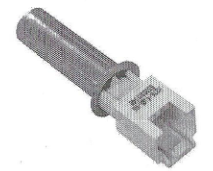
\includegraphics[width=0.3\linewidth]{sonda-termica}
\centering
\end{minipage}

Es una resistencia variable por temperatura, según el modelo, su resistencia aumentará o disminuirá con la temperatura.
Se encuentran en diferentes formas en una gran variedad de electrodomésticos.
El modelo de la foto se encuentra en algunas lavadoras.
\\

Está conectado principalmente a una tarjeta electrónica que controla la
temperatura.

En general, si se obtiene un valor de resistencia que no sea ni cortocircuito ni infinito, hay muchas posibilidades de que el sensor esté en buen estado.
En el caso de sensores en contacto con el agua, como éste, la cal adherida al sensor 
puede ser responsable de un problema de regulación de la temperatura.
En este caso, basta con limpiarlo con vinagre blanco.
\end{normalize}

\end{itemize}
\newpage
\begin{center}
\textbf{c) Sensores de posición por campo magnético}
\end{center}
Se encuentran a menudo en electrodomésticos, para detectar la presencia de agua en un depósito (cafetera, plancha, ...) o captar la posición del tambor en una lavadora.\\


Hay dos grandes familias:

\begin{itemize}
\item Los sensores "ILS", que funcionan como un interruptor abierto o cerrado según la presencia de un imán a proximidad.

\begin{figure}[h]
\centering
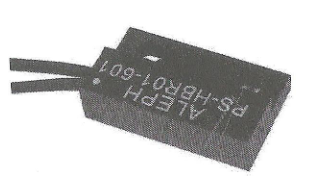
\includegraphics[width=0.6\linewidth]{sensor-ILS}
\caption*{\textit{Tipo "ILS": Sensor de posición del tambor de una lavadora}}
\end{figure}

\item Los sensores de "efecto hall", que hacen variar la tensión de sus contactos según la intensidad del campo magnético a proximidad.

\begin{figure}[h]
\centering
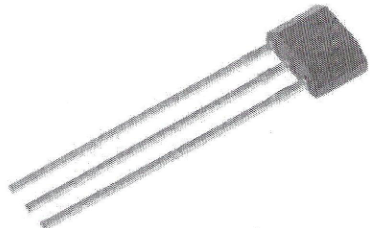
\includegraphics[width=0.6\linewidth]{sensor-hall}
\caption*{\textit{Tipo "efecto hall"}}
\end{figure}

\end{itemize}
\newpage 

\begin{center}
\textbf{d) Sensores de presión (presostatos)}
\end{center}
Se pueden encontrar en lavadoras, generadores de vapor, lavadoras, máquinas expreso.... Constan de 1, 2 o incluso 3 conmutadores "común - reposo/trabajo" que conmutan en función de la presión que reciben.

\noindent\begin{minipage}[t]{0.4\textwidth}\vspace{0pt}
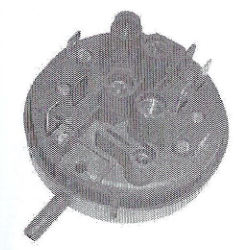
\includegraphics[width=\linewidth]{sensor-presion}
Presostato de una lavadora
\end{minipage}
\hfill%
\begin{minipage}[t]{0.5\textwidth}\vspace{\fill}
\vspace{\fill}
En el caso de los presostatos de las
lavadoras, la presión es una imagen del nivel de
nivel de agua en la máquina.
Los nombres de las clavijas suelen ser
así:
\\

Dígito de las decenas: nivel de agua (1 para
$1^{er}$ nivel...)
Dígito de las unidades: 1: común / 2 :
resto / 3: trabajo\\
\vspace{\fill}
\end{minipage}
\vspace{1em}

\begin{figure}[h]
\centering
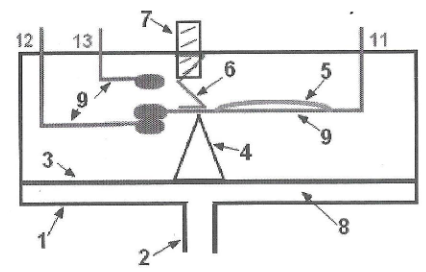
\includegraphics[width=0.6\linewidth]{esquema-presostato}
\caption*{\textit{Esquema de un presostato}}
\end{figure}

\textbf{Funcionamiento:\\}
En reposo, el muelle "6" hace contacto entre "11" y "12".
el aire comprimido por el agua del depósito llega a "2", presiona sobre la membrana
membrana "3" y después sobre la aguja "4".
El efecto de esta presión es forzar a la lengüeta "9", conectada a "11", a 
desconectarse de "12" y conectarse a "13".

\end{document}